\documentclass[11pt,a4paper]{article}
% \usepackage{footnote}
% \makesavenoteenv{tabular}
\usepackage[hyperref]{emnlp2018}
\usepackage{times}
\usepackage{latexsym}
\usepackage{amsmath}
\usepackage{amssymb}
\usepackage{graphicx,subcaption}
\usepackage{float}
\usepackage{nicefrac}

\usepackage{framed}
\usepackage{longtable}
\usepackage{url}
\usepackage{hyperref}

\newcommand\BibTeX{B{\sc ib}\TeX}
% \newcommand\conforg{SIGDAT}

\DeclareMathOperator*{\argmax}{arg\,max}
\DeclareMathOperator*{\argmin}{arg\,min}

\title{Sequence-to-sequence Machine Translation Report}

\author{Ethan Xuanyue Yang \\
%   Affiliation / Address line 1 \\
%   Affiliation / Address line 2 \\
%   Affiliation / Address line 3 \\
  {\tt xuanyuey@cs.cmu.edu}}

% \date{}

\begin{document}
\maketitle
% \begin{abstract}
%   This document contains the instructions for preparing a camera-ready
%   manuscript for the proceedings of \confname{}. The document itself
%   conforms to its own specifications, and is therefore an example of
%   what your manuscript should look like. These instructions should be
%   used for both papers submitted for review and for final versions of
%   accepted papers.  Authors are asked to conform to all the directions
%   reported in this document.
% \end{abstract}

\section{Introduction}

In this report we present the implementation (\href{https://github.com/YangXuanyue/mt-hw1-encoder-decoder}{Github}) of an RNN-based sequence-to-sequence model for machine translation, composed an encoder for source sentence and a decoder with attention over source encodings for target sentence. We conduct a series of experiment and show the effectiveness of our settings of certain hyper-parameters by the comparison of BLEU scores. We then discuss several factors that show influence on the performance.

\section{Model}
The model has a classic encoder-decoder architecture to translate a source sentence into a target sentence.
\subsection{Encoder}
We first use a source embedding matrix $\mathbf{E}_\text{src}\in\mathbb{R}^{V_\text{src}\times D}$, where $V_\text{src}$ is source vocabulary size, $D$ z to embed the input tokenized source sentence $\{x_t\}_{t=1}^{T_\text{src}}$ (word ID sequence) to $\{\mathbf{x}_t\}_{t=1}^{T_\text{src}}$. Then we use an $L$-layer bidirectional $\mathrm{LSTM}_\text{src}$ to encode it:
\begin{align}
    \overrightarrow{\mathbf{h}}^\text{src}_{l,t} &= \overrightarrow{\mathrm{LSTM}}_\text{src}(\mathbf{h}^\text{src}_{l-1,t}, \overrightarrow{\mathbf{h}}^\text{src}_{l,t-1}),\\
    \overleftarrow{\mathbf{h}}^\text{src}_{l,t} &= \overleftarrow{\mathrm{LSTM}}_\text{src}(\mathbf{h}^\text{src}_{l-1,t}, \overleftarrow{\mathbf{h}}^\text{src}_{l,t+1}), \\
    \mathbf{h}^\text{src}_{l,t} &= \begin{bmatrix}
    \overrightarrow{\mathbf{h}}^\text{src}_{l,t} \\
    \overleftarrow{\mathbf{h}}^\text{src}_{l,t}
  \end{bmatrix},
\end{align}
where
\begin{align}
    \overrightarrow{\mathbf{h}}^\text{src}_{l,0} &= \overleftarrow{\mathbf{h}}^\text{src}_{l,T_\text{src}+1} = \mathbf{0}, \\
    \mathbf{h}^\text{src}_{0,t} &= \mathbf{x}_t.
\end{align}
Eventually we obtain source encoding matrices for each layer:
\begin{align}
    \mathbf{H}^\text{src}_l = \begin{bmatrix}
    \mathbf{h}^\text{src}_{l,1}, \cdots,
    \mathbf{h}^\text{src}_{l,T_\text{src}}
    \end{bmatrix}.
\end{align}
\subsection{Decoder}
Given a target sentence $\{y_t\}_{t=1}^{T_\text{tgt}}$, similarly we use a target embedding matrix $\mathbf{E}_\text{tgt}\in\mathbb{R}^{V_\text{tgt}\times D}$ to embed it to $\{\mathbf{y}_t\}_{t=1}^{T_\text{tgt}}$. Then an $L$-layer $\mathrm{LSTM}_\text{tgt}$ serve as target language model along with attentional contexts over the source encodings:
\begin{align}
    \mathbf{h}^\text{tgt}_{l,t} = \mathrm{LSTM}_\text{tgt}\left(
    \begin{bmatrix}
    \mathbf{h}^\text{tgt}_{l,t} \\
    \mathbf{c}_{l,t-1}
    \end{bmatrix}, \mathbf{h}^\text{tgt}_{l,t-1}
    \right),
\end{align}
where
\begin{align}
    \mathbf{h}^\text{tgt}_{l,0} &= \begin{bmatrix}
    \overrightarrow{\mathbf{h}}^\text{src}_{l,T} \\
    \overleftarrow{\mathbf{h}}^\text{src}_{l,0}
  \end{bmatrix}, \\
    \mathbf{h}^\text{tgt}_{0,t} &= \mathbf{y}_t.
\end{align}
We feed the previous context $\mathbf{c}_{l,t}$ as a part of input at $t$ to inform the decoder of previous alignment decision similar to \citet{luong2015effective}. Each $\mathbf{c}_{l,t}$ is obtained using scaled dot product attention \cite{vaswani2017attention}:
\begin{align}
    \mathbf{a}_{l,t} &= (\mathrm{softmax}(\mathbf{q}_{l,t}^\mathsf{T}\mathbf{K}_l))^\mathsf{T}, \\
    \mathbf{c}_{l,t} &= \frac{1}{\sqrt{H}}\mathbf{V}_l\mathbf{a}_{l,t},
\end{align}
where $H$ is the hidden size, and the query $\mathbf{q}_{l,t-1}$, keys $\mathbf{K}_l$, and values $\mathbf{V}_l$ is computed by:
\begin{align}
    \mathbf{q}_{l,t} = \text{MLP}_\text{q}(\mathbf{h}_{l,t}), \\
    \mathbf{K}_l = \text{MLP}_\text{k}(\mathbf{H}^\text{src}_l), \\
    \mathbf{V}_l = \text{MLP}_\text{v}(\mathbf{H}^\text{src}_l).
\end{align}

Finally we project the $L$-th target encodings and contexts to a $V_\text{tgt}$-dimensional logit vector, and $\mathrm{softmax}$ it with temperature $T$ as the predicted probability distribution over the target vocabulary:
\begin{align}
    &\mathbf{o}_t = \mathrm{tanh}\left(\mathbf{W}_\text{o}\begin{bmatrix}
    \mathbf{h}^\text{tgt}_{L,t} \\
    \mathbf{c}_{L,t}
    \end{bmatrix}
    \right), \\
    &\mathbf{s}_t = \mathbf{W}_\mathrm{tgt}\mathbf{o}_t, \\
    &\hat{\mathbf{p}}_t = \mathrm{softmax}\left(\frac{\mathbf{s}_t}{T}\right), \\
    &\mathbb{P}(y|\{x_\tau\}_{\tau=1}^{T_\text{src}},\{y_\tau\}_{\tau=1}^{t-1}) = \hat{\mathbf{p}}_t[y].
\end{align}
We apply weight tying \cite{press2016using} to regularize target projection and embedding matrix by enforcing $\mathbf{W}_\mathrm{tgt}=\mathbf{E}_\mathrm{tgt}$.
\subsection{Training Process} \label{tp}
During training time we have the gold target sentence and thus we maximize the log-likelihood of it given by the model, or equivalently the cross entropy:
\begin{align}
    \mathcal{L} = \sum_{t=1}^{T_\text{tgt}}\log\mathbb{P}(y_t|\{x_\tau\}_{\tau=1}^{T_\text{src}},\{y_\tau\}_{\tau=1}^{t-1}).
\end{align}

Generally in an encoder-decoder model
we have a discrepancy between training and inference, specifically the decoder has access to the previous gold word when making sequential predictions during the former, while lacks it during the latter. To bridge this gap we occasionally feed the decoder with the previous predicted word $\hat{y}_{t-1}$ instead of the gold word $y_{t-1}$, similar to scheduled sampling \cite{bengio2015scheduled} but we are using a constant rate $R$. An issue comes consequently is the exploration-exploitation trade-off: trivially feeding the
\begin{align}
    \hat{y}_{t-1}=\argmax_y\mathbb{P}(y|\{x_\tau\}_{\tau=1}^{T_\text{src}},\{y_\tau\}_{\tau=1}^{t-1})
\end{align}
might cause the sequential decisions to be stuck in local optima and even misled when the model is not well-trained yet. We thus change the deterministic $\argmax_y$ to a sampling:
\begin{align}
    \Tilde{y}_{t-1}\sim \mathbb{P}(y|\{x_\tau\}_{\tau=1}^{T_\text{src}},\{y_\tau\}_{\tau=1}^{t-1})
\end{align}
and feed $\Tilde{y}_{t-1}$ as input to explore more possibilities. With the help of the straight-through Gumbel-softmax re-parameterization trick \cite{jang2016categorical} we are able to do continuous optimization through these sampling step and over each decision $\hat{\mathbf{p}}_{t-1}$. Specifically the sampling could be reparameteriazed by a Gumbel distribution:
\begin{align}
    &g_i\overset{\text{i.i.d.}}{\sim}\mathrm{Gumbel}(0,1), i = 1,\dots,V_\text{tgt} \\
    &\Tilde{\mathbf{p}}_{t-1} = \mathrm{softmax}\left(\frac{\mathbf{s}_{t-1}+\mathbf{g}}{T}\right), \\
    &\Tilde{y}_{t-1} = \argmax_y \Tilde{\mathbf{p}}_{t-1},
\end{align}
and we use $\mathbf{E}_\text{tgt}\Tilde{\mathbf{p}}_{t-1}$ to calculate the gradient in the backward pass, but use $\Tilde{y}_{t-1}$ in the forward pass to avoid propagating mixing errors due to feeding a mixture of word embeddings \cite{gu2018neural}.

\subsection{Decoding Process}
Searching the best target sequence is essentially an exponential process and we use beam search to obtain a sub-optimal result in a polynomial space. With a beam size $B$, we start by feeding the start token \texttt{<s>} to the decoder and at each step $t>1$ we have $B$ target sequences as inputs. For each sequence we keep top $B$ next words out of $V_\text{tgt}$, and then we keep top $B$ new sequences out of $BV_\text{tgt}$. For ranking we consider the length-normalized log-likelihood of each sequence $\{\hat{y}_\tau\}_{\tau=1}^t$:
\begin{align}
    l(\{\hat{y}_\tau\}_{\tau=1}^t) &= \sum_{\tau=1}^t \mathbb{I}(\hat{y}_\tau\neq\mathrm{id}(\texttt{</s>})),\\
    s(\{\hat{y}_\tau\}_{\tau=1}^t) &= \frac{\sum_{\tau=1}^{t}\log\mathbb{P}(\hat{y}_t|\{x_\tau\}_{\tau=1}^{T_\text{src}},\{\hat{y}_\tau\}_{\tau=1}^{t-1})}{l(\{\hat{y}_\tau\}_{\tau=1}^t)},
\end{align}
where we enforce the decoder to only predict \texttt{</s>} for a sequence ended with \texttt{</s>}. Either when each of the $B$ sequences has ended or maximum decoding length $T_\text{max}$ has been reached we terminate the decoding and choose the highest-scored sequence as the result.

\section{Experiment}
\subsection{Dataset}
We use the IWSLT 2014 de-en dataset\footnote{https://wit3.fbk.eu/mt.php?release=2014-01}\cite{cettolo2012wit3}, which has 150K German-English training sentences. We use the pre-processed version of the training set from \citet{ranzato2015sequence} with long sentences chopped and rared words replaced by a special \texttt{<unk>} token and use the original validation and test sets. Wu build the source and target vocabularies out of the training set with words of frequency more than 2, resulting in sizes $V_\text{src}=22824$ and $V_\text{tgt}=32011$.
\subsection{Settings}
We list our experiment settings for the best model in Table~\ref{settings}. For $\mathrm{LSTM}_\text{src}$ we use $\nicefrac{H}{2}$ per each direction. We also consider a RNN weight dropout probability for weight-dropped RNN \cite{merity2017regularizing} where a fixed dropout mask is applied to RNN weights at each time step per run, though in the final model we cancel this setting due to its unpromising performance as shown in Table \ref{results}. During training we reduce the learning rate by half and reload the previous model checkpoint each time we have seen a non-increasing validating perplexity after 1 patient step. We do early-stopping after 4 times of adjusting the learning rate but not witnessing improvement.
\begin{table}
\centering
\begin{tabular}{lll}
  \textbf{Item} & \textbf{Value} \\
  \hline
  Embedding Dimension $D$ & 512 \\
  RNN Hidden Size $H$ & 512 \\
  \#(RNN Layer) $L$  & 2 \\
  Temperature $T$ & 0.5 \\
  Sampling Rate $R$ & 0.2 \\
  Dropout Probability & 0.2 \\
  RNN Weight Dropout Probability & 0 \\
  Optimizer & Adam \\
  Initial Learning Rate & $10^{-3}$ \\
  Batch Size & 64 \\
  Beam Size $B$ & 32 \\
  Max Decoding Length $T_\text{max}$ & 200
\end{tabular}
\caption{Settings}
\label{settings}
\end{table}
\subsection{Results}
We report the results in terms of validating perplexity (ppl.), validating BLEU and test BLEU\footnote{calculated by \hyperlink{https://github.com/moses-smt/mosesdecoder/blob/master/scripts/generic/multi-bleu.perl}{multi-bleu.perl}} in Table \ref{results}, where we start from a ``Base'' 1-layer RNN model and gradually apply several changes. We use validating perplexity for model selection.
\begin{table}[!htbp]
\centering
\begin{tabular}{l|c|c|c}
  \textbf{Model} & \textbf{Val} & \textbf{Val.} & \textbf{Test} \\
  & \textbf{Ppl.} & \textbf{BLEU} & \textbf{BLEU} \\
  \hline
  Base & 9.11 & 29.65 & 27.61 \\
  $+$ Weight Dropping & 9.35 & 29.12 & 27.03 \\
  2-Layer & 8.85 & 29.99 & 27.75 \\
  ~~$+$Sampling  & 8.74 & 29.79 & 27.78 \\
  ~~~~\textbf{$+$Weight Tying} & \textbf{8.54} & \textbf{30.12} & \textbf{28.01} \\

\end{tabular}
\caption{Results}
\label{results}
\end{table}
\subsection{Analysis}

From the experiment result we mainly find three changes that are particularly helpful for improving the performance. The number of RNN Layer, weight tying and sampling (see \ref{tp}). We have also tried weight dropping for RNNs but the eventually the converged model gives both a higher training and validation perplexity, suggesting that under the current settings we have, applying dropout on RNN weights act as a too strong regularization and potentially hinder the learning of the model. As shown effective in generalizing the RNN-based language models in \citet{merity2017regularizing}, this method might further improve our performance given more sophisticated hyper-parameter tuning.

Increasing the number of RNN layers is both a trivial and heavy-weight change, as it greatly increase the step time and GPU usage of the model. Its improvement could mainly be attributed to enable to model to consider higher-level information by adding the depth of the RNN-encoding layer. Intuitively the second layer of the encoder might render more informative word encodings based on the first layer encodings. And the second layer of the decoder might be able to make better prediction decision by considering the adjusting the decision from the first layer.

We plot the convergence processes in terms of training and validating perplexity for the 2-layer model and models we apply sampling and weight tying in Fig. \ref{ppls}. We would discuss the effect of adding sampling and weight tying below.

\begin{figure}
  \centering
  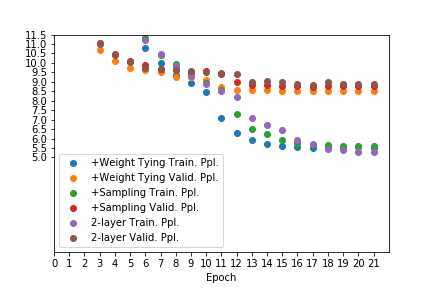
\includegraphics[width=0.55\textwidth]{ppls.png}
  \caption{Training and Validating Perplexity vs Epoch}
  \label{ppls}
\end{figure}


As discussed before, sampling would help reducing the training-inference discrepancy by simulating the decoding behaviour in the training time, ie, feeding the output from the previous time step as current input. These sampling steps would intuitively result in slower initial convergence rate for training when the model is not well-trained and have higher loss for making decision out of a non-gold input. This phenomenum is well reflected in Fig. \ref{ppls} where for the first 10 epochs the training and validating perplexities are higher than others. But after this phase the model starts to achieve better performance than its simpler 2-layer peer. And eventually the model could have higher validating and test BLEU score due to these decoding steps have been more or less exposed in training time.

The last and the most significant improvement we make is by applying weight tying. From the convergence curves we could that it constantly achieves a better training and validating perplexities over others, and converges faster (4-5 epochs less). And it greatly
increase the test BLEU by 0.23, more than that brought by deepening RNNs (0.14). We conjecture that tying the weights for the embedding matrix and the projection matrix informs the model to directly utilize the word embedding similarities for word prediction, and in turn force the model to learn more task-specific embeddings. Also without learning two large weight matrices, the model enjoys a simpler structure and thus converges faster. It's interesting that this regularization technique would result in both faster convergence of training and validating perplexity, thanks to its reasonable simplification without hurting the model's capability to make prediction in training time, compared to dropout.


\begin{table}[!htbp]
\centering
\begin{tabular}{l|c|c|c}
  \textbf{Frequency} & \textbf{+W.T.} & +S.& 2-Layer  \\
  \hline
  $<1$ & 0 & 0 & 0 \\
  $1$ & \textbf{0.280} &  0.272 & 0.270 \\
  2 &  \textbf{0.392} & 0.387 & 0.383  \\
3 &  \textbf{0.424} & 0.421 & 0.417 \\
4  & 0.442 & \textbf{0.444} & 0.439 \\
$[5,10)$ & \textbf{0.508} & 0.503 & 0.497 \\
$[10,100)$   & 0.56 & \textbf{0.572} & 0.569 \\
$[100,1000)$ &  \textbf{0.603} & 0.601 & 0.600 \\
$\ge1000$ & \textbf{0.753} & 0.753 & 0.750 \\

\end{tabular}
\caption{Word F-measures}
\label{fmes}
\end{table}

\begin{table}[!htbp]
\centering
\begin{tabular}{l|c|c|c}
  \textbf{Length} & \textbf{+W.T.} & +S.& 2-Layer  \\
  \hline
  $<10$ &\textbf{32.78}& 32.27 &32.84 \\
$[10,20)$ &30.29 &\textbf{30.44} &30.18 \\
$[20,30)$ &\textbf{28.22} &28.13 &27.77 \\
$[30,40)$ &\textbf{26.58} &25.98 &25.93 \\
$[40,50)$ &\textbf{25.72} &25.20 &25.28 \\
$[50,60)$ &\textbf{24.68} &23.81 &24.51 \\
$\ge60$   & 20.61 &\textbf{20.71}& 21.62 \\
\end{tabular}
\caption{Sentence BLEUs}
\label{sbs}
\end{table}

We further use \texttt{compare-mt} \cite{neubig19naacl} to  compute the word F-measures bucketed by word frequency and sentence BLEUs bucketed by sentence length. As shown in Table \ref{fmes} and \ref{sbs}, where ``+W.T.'' is our best model with weight tying, ``+S.''the one with only sampling, and ``2-Layer'' the one without both, weight tying and sampling consistently give better results than the simple 2-layer version, but weight tying is outperformed by just sampling in some cases. This could be because weight tying is a hard regularization and a more complex model with more parameters without it would be able to cover some special cases. Overall weight tying still delivers the best result, in terms of predicting the correct words and composing the sentences relevant to the references.


\begin{table}[!htbp]
\centering
\begin{tabular}{l|l}
\hline
Ref.& this is a game for outside. \\
\textbf{+W.T.}& \textbf{this is a game for outside.}\\
+S.& that's a game out there.\\
\hline
Ref.& the mechanism comes from the lie.\\
\textbf{+W.T.}& \textbf{the mechanism comes from the lie.}\\
+S.& the mechanism is from lie.\\
\hline
Ref.& so where do we go?\\
\textbf{+W.T.}& \textbf{so where do we go?}\\
+S.& so where are we going?\\
\hline
Ref.& and i think it makes the world look like this.\\
\textbf{+W.T.}& \textbf{and i think it makes the world look like this.}\\
+S.& and i think it's a sense of the world looks like this.\\
\hline
Ref.& imagine a plane full of smoke.\\
\textbf{+W.T.}& \textbf{imagine a plane full of smoke.}\\
+S.& imagine a plane full of a fish.\\
\hline
Ref.& the orange tractor.\\
+W.T.& the orange is $<$unk$>$.\\
\textbf{+S.}& \textbf{the orange tractor.}\\
\hline
Ref.& but it gets worse.\\
+W.T.& but it's even worse.\\
\textbf{+S.}& \textbf{but it gets worse.}\\
\hline
Ref.& i'm going to stop that.\\
+W.T.& i'll stop that.\\
\textbf{+S.}& \textbf{i'm going to stop that.}\\
\hline
Ref.& it's kind of like a potato.\\
+W.T.& it's about a potato.\\
\textbf{+S.}& \textbf{it's kind of like a potato.}\\
\hline
Ref.& if you burn natural gas, no.\\
+W.T.& if you burn gas , you're not.\\
\textbf{+S.}& \textbf{if you burn natural gas, no}\\
\hline

\end{tabular}
\caption{Translation Examples}
\label{tx}
\end{table}


At last we showcase several translation examples produced by \texttt{compare-mt} \cite{neubig19naacl} in Table \ref{tx}, where the first 5 our best model with weight typing wins, and the last 5 the one with just sampling wins. We could see that overall our best model is able to generate more fluent sentences and cover the basic meaning, even in loss cases. While in some loss cases for the model without weight tying, sentences that are slightly incorrect such as ``and i think it's a sense of the world looks like this.'', and also sentences that are far off the references such as ``imagine a plane full of a fish.'' are generated.

\bibliography{emnlp2018}
\bibliographystyle{acl_natbib_nourl}


\end{document}
